\section{Preliminary Out-of-Plane Scour Scenario}
\label{sec:dmem-scour-out-of-plane}

A preliminary three-dimensional analysis is also introduced to examine support loss across the bridge width. In this case, scour is applied to the upstream part of the foundation and is described by the transverse support-loss ratio $\eta_{s,y}$. The objective at this stage is qualitative: to verify that the model can represent the expected out-of-plane deformation pattern and the associated redistribution of interface stresses. Numerical capacity indicators from this scenario still require a separate post-processing and verification step before they can be compared with the in-plane residual-capacity curves.

\subsection{Collapse Progression}
\label{sec:dmem-scour-out-of-plane-collapse}

\Cref{fig:dmem-scour-out-of-plane-phases} shows the deformation sequence for increasing transverse scour. The 3D view gives the global mechanism, while the XZ and YZ projections separate the longitudinal and transverse components of the response.

\begin{figure}[htbp]
\centering
\setlength{\tabcolsep}{2pt}
\renewcommand{\arraystretch}{1.1}

\begin{tabular}{c c c c}
 & \textbf{3D} & \textbf{XZ} & \textbf{YZ} \\

\textbf{Vert} &
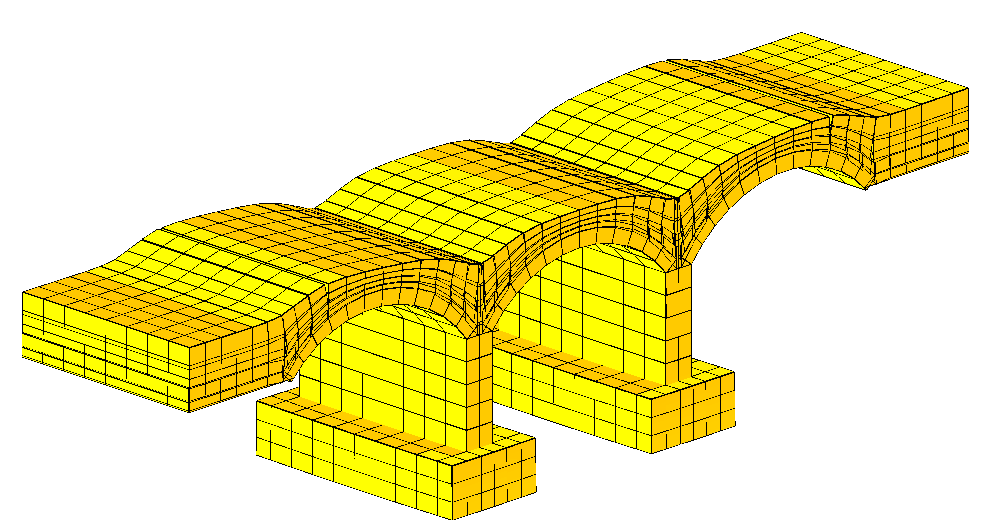
\includegraphics[width=0.28\textwidth]{./Figures/out_of_plane_scour_phases/3D/vert_3D.png} &
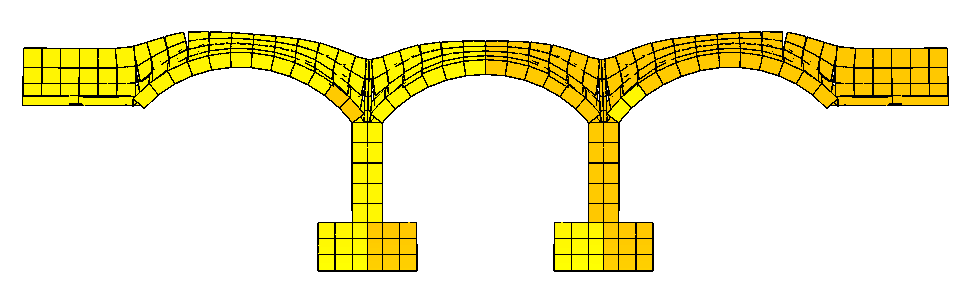
\includegraphics[width=0.28\textwidth]{./Figures/out_of_plane_scour_phases/XZ/vert_XZ.png} &
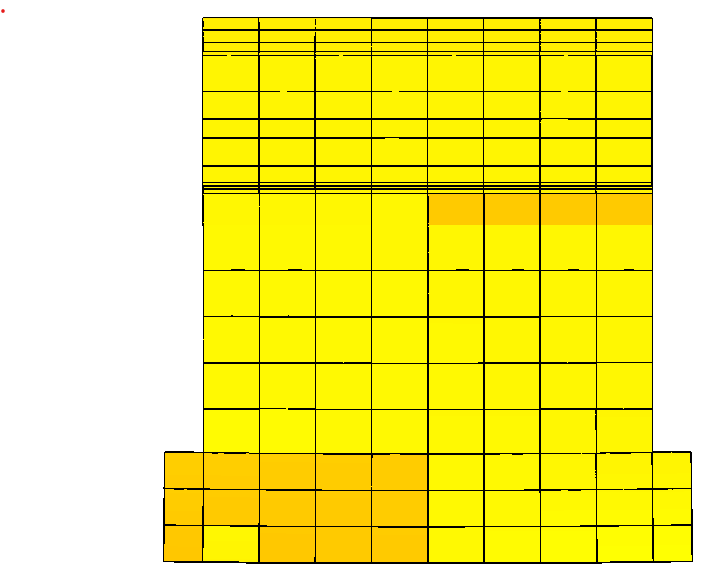
\includegraphics[width=0.28\textwidth]{./Figures/out_of_plane_scour_phases/YZ/vert_YZ.png} \\

\textbf{Scour 1} &
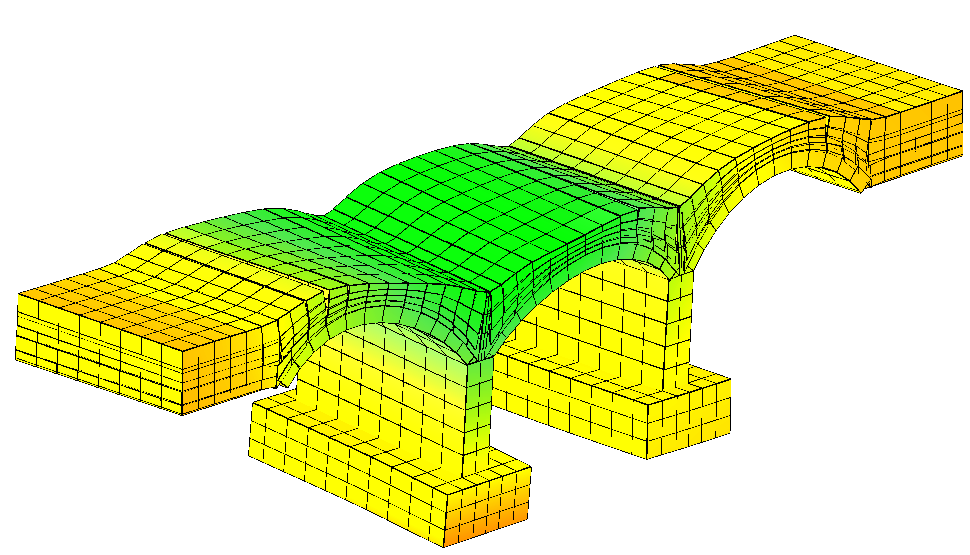
\includegraphics[width=0.28\textwidth]{./Figures/out_of_plane_scour_phases/3D/scour1_3D.png} &
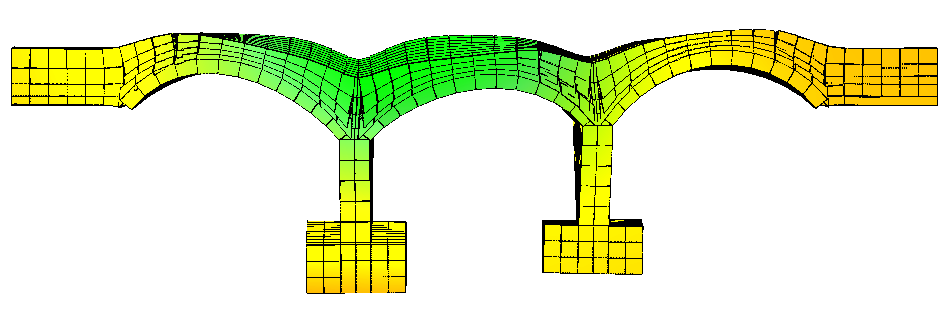
\includegraphics[width=0.28\textwidth]{./Figures/out_of_plane_scour_phases/XZ/scour1_XZ.png} &
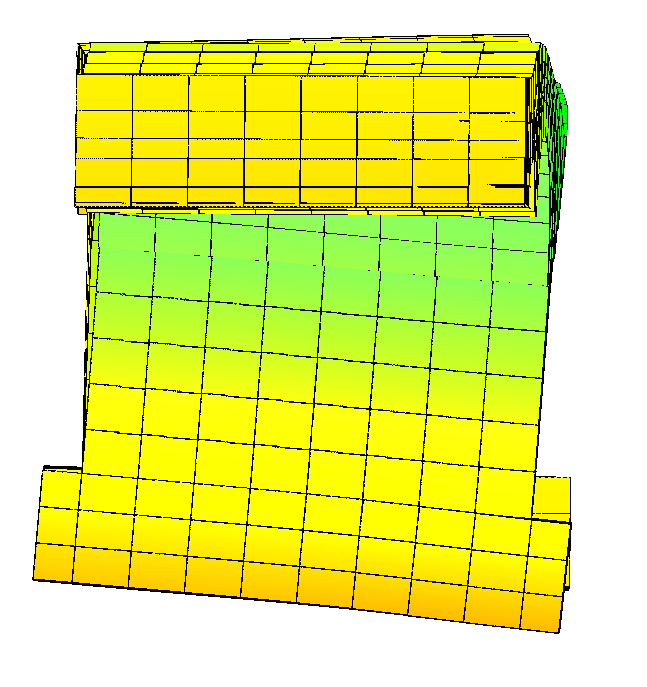
\includegraphics[width=0.28\textwidth]{./Figures/out_of_plane_scour_phases/YZ/scour1_YZ.png} \\

\textbf{Scour 2} &
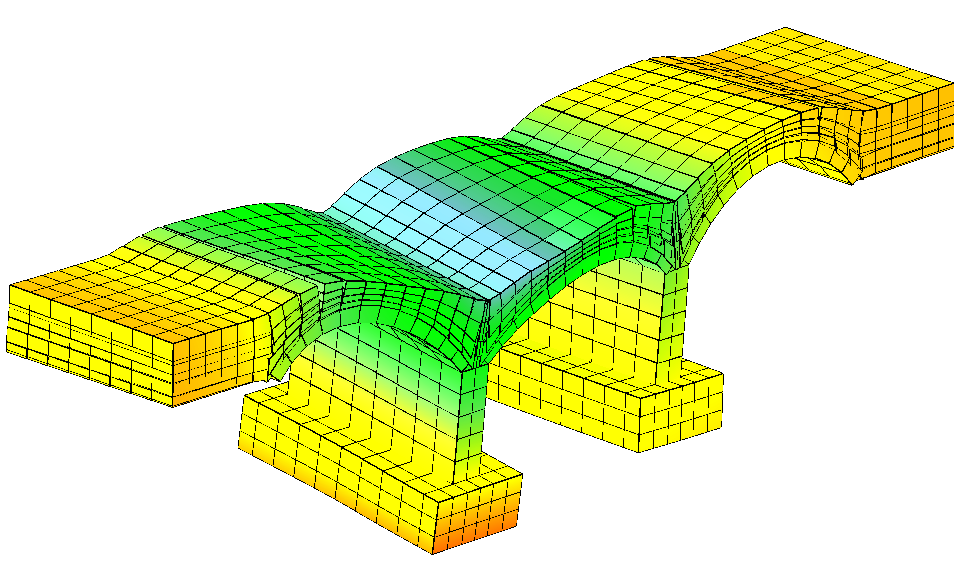
\includegraphics[width=0.28\textwidth]{./Figures/out_of_plane_scour_phases/3D/scour2_3D.png} &
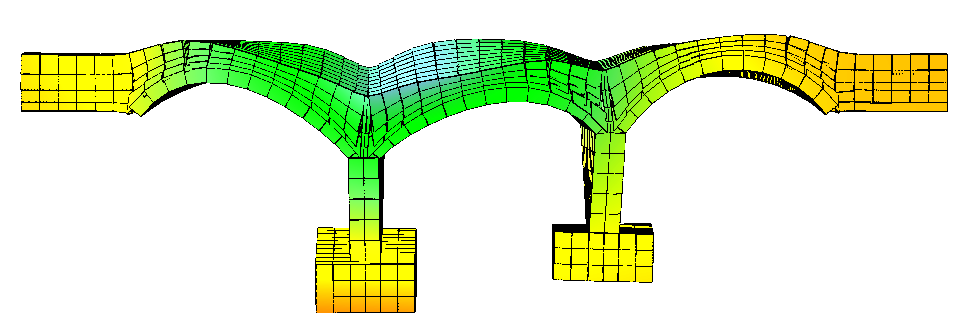
\includegraphics[width=0.28\textwidth]{./Figures/out_of_plane_scour_phases/XZ/scour2_XZ.png} &
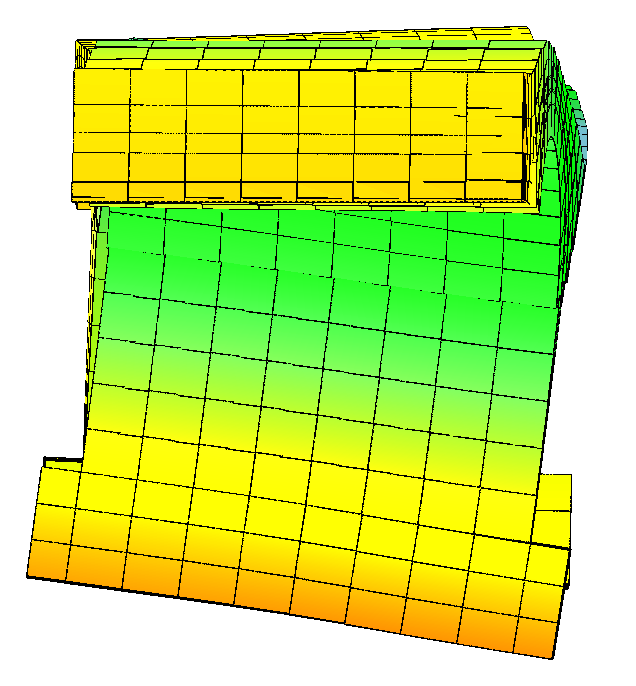
\includegraphics[width=0.28\textwidth]{./Figures/out_of_plane_scour_phases/YZ/scour2_YZ.png} \\

\textbf{Scour 3} &
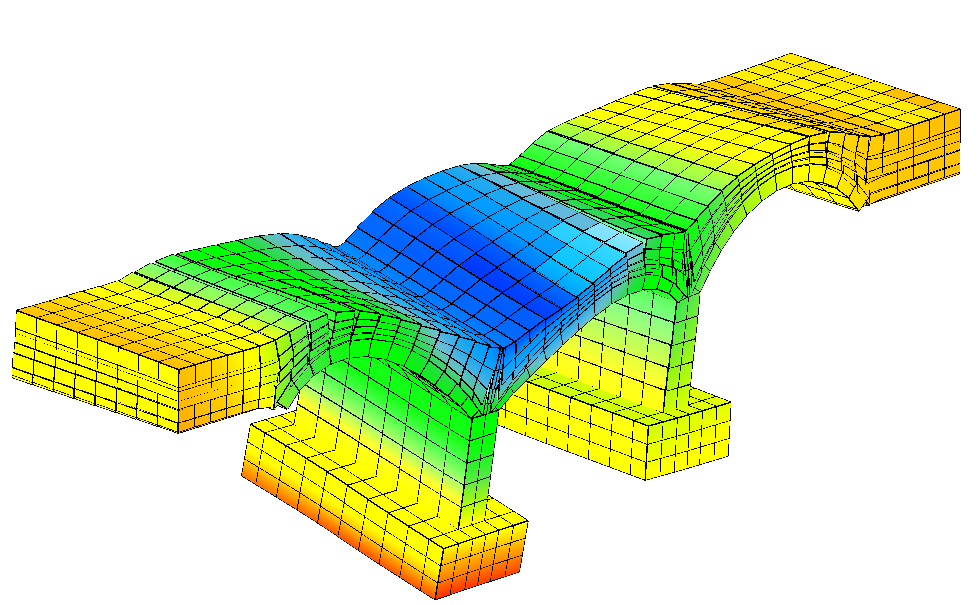
\includegraphics[width=0.28\textwidth]{./Figures/out_of_plane_scour_phases/3D/scour3_3D.png} &
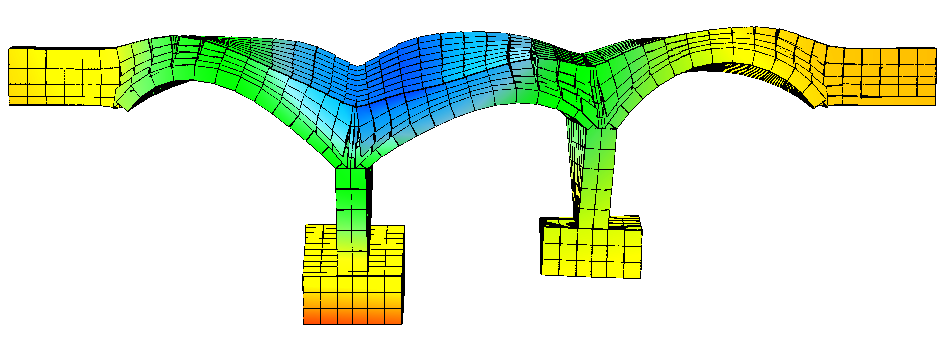
\includegraphics[width=0.28\textwidth]{./Figures/out_of_plane_scour_phases/XZ/scour3_XZ.png} &
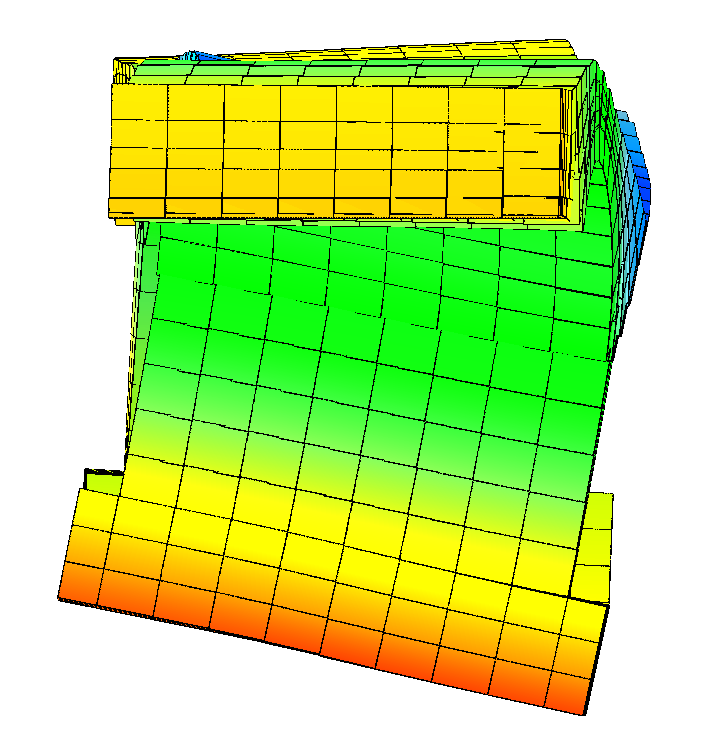
\includegraphics[width=0.28\textwidth]{./Figures/out_of_plane_scour_phases/YZ/scour3_YZ.png} \\

\textbf{Scour 4} &
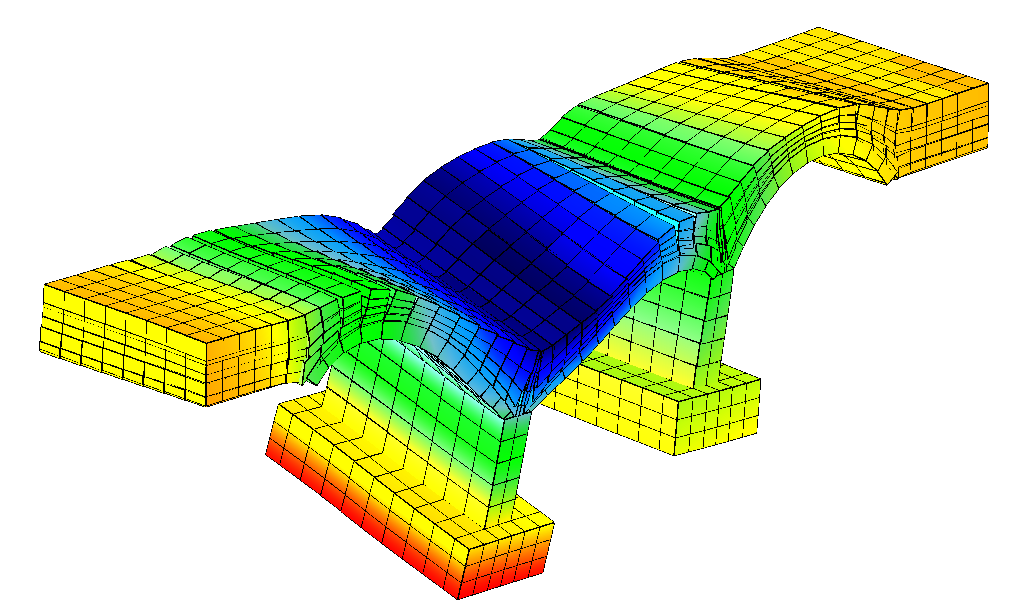
\includegraphics[width=0.28\textwidth]{./Figures/out_of_plane_scour_phases/3D/scour4_3D.png} &
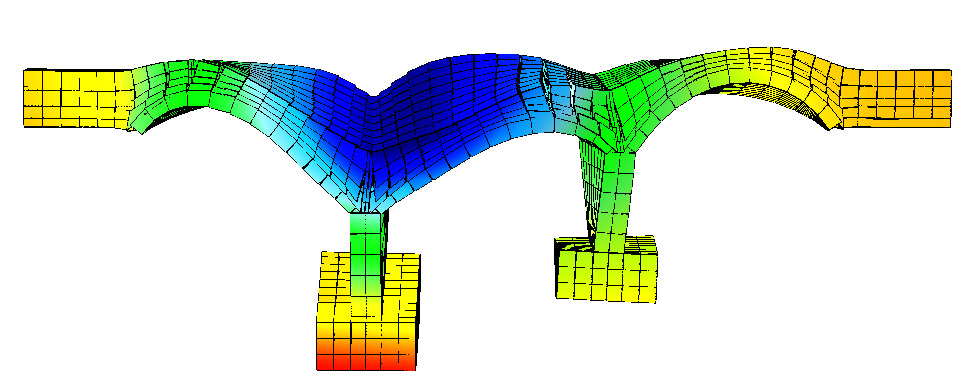
\includegraphics[width=0.28\textwidth]{./Figures/out_of_plane_scour_phases/XZ/scour4_XZ.png} &
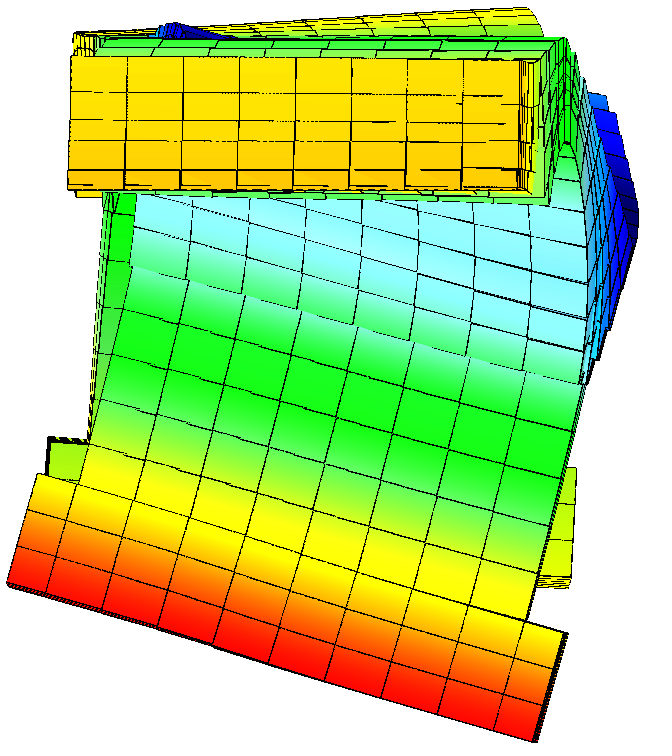
\includegraphics[width=0.28\textwidth]{./Figures/out_of_plane_scour_phases/YZ/scour4_YZ.png} \\

\end{tabular}

\caption{Preliminary out-of-plane scour phases shown in 3D, XZ, and YZ views.}
\label{fig:dmem-scour-out-of-plane-phases}
\end{figure}

\subsection{Interface Stress Redistribution}
\label{sec:dmem-scour-out-of-plane-stresses}

\Cref{fig:dmem-scour-out-of-plane-interface-stress} shows the corresponding interface-stress fields. The plots distinguish the overall interface stress from the tensile and compressive components so that stress concentration and unloading zones can be checked separately.

\begin{figure}[htbp]
\centering
\setlength{\tabcolsep}{4pt}
\renewcommand{\arraystretch}{1.1}

\begin{tabular}{c c c}
 & \textbf{3D} & \textbf{XY top view} \\

\textbf{Interface stress} &
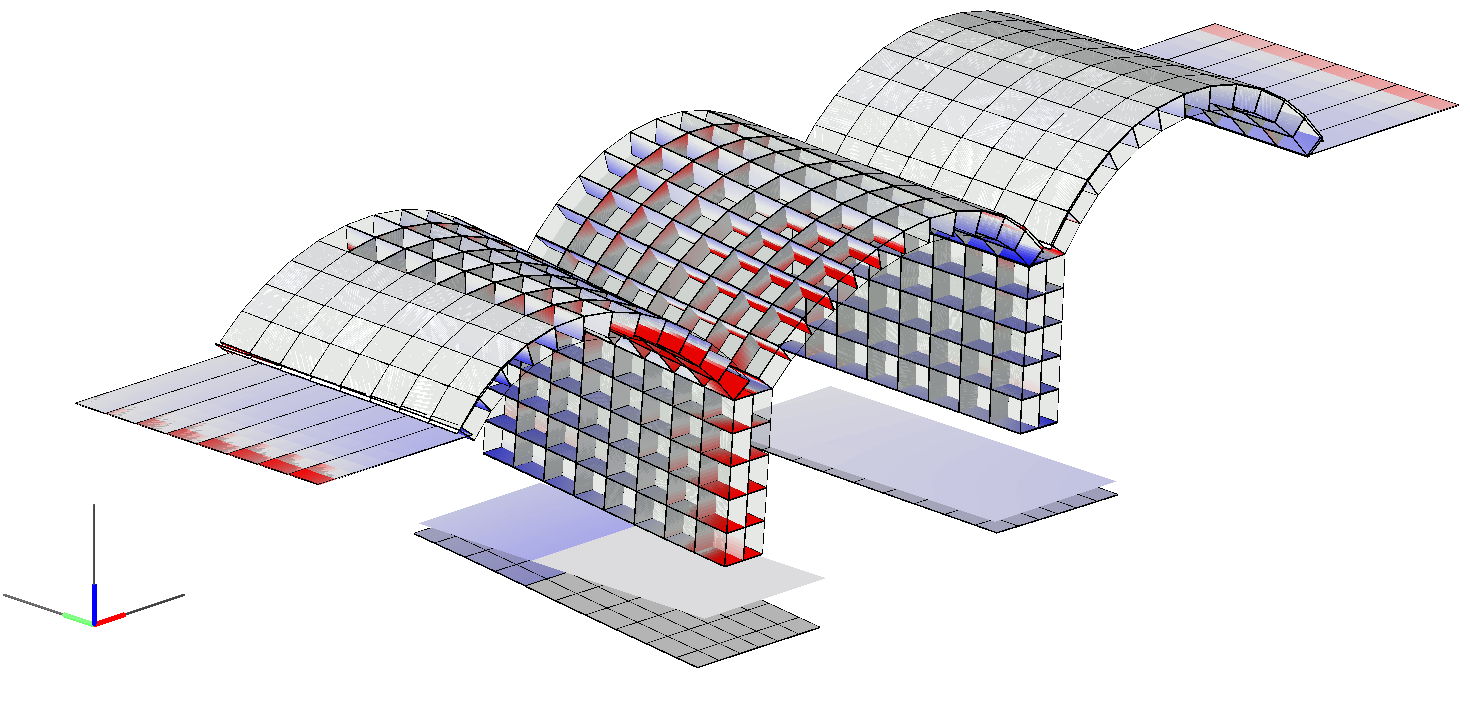
\includegraphics[width=0.42\textwidth]{./Figures/out_of_plane_scour_phases/stresses/interface_stress_3D.png} &
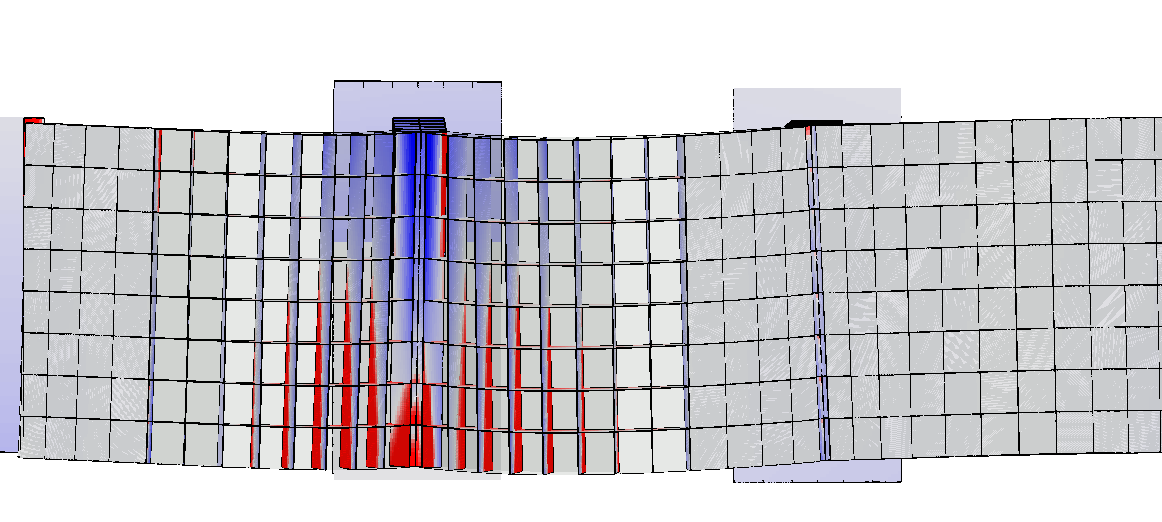
\includegraphics[width=0.42\textwidth]{./Figures/out_of_plane_scour_phases/stresses/interface_stress_XY_topview.png} \\

\textbf{Tensile stress} &
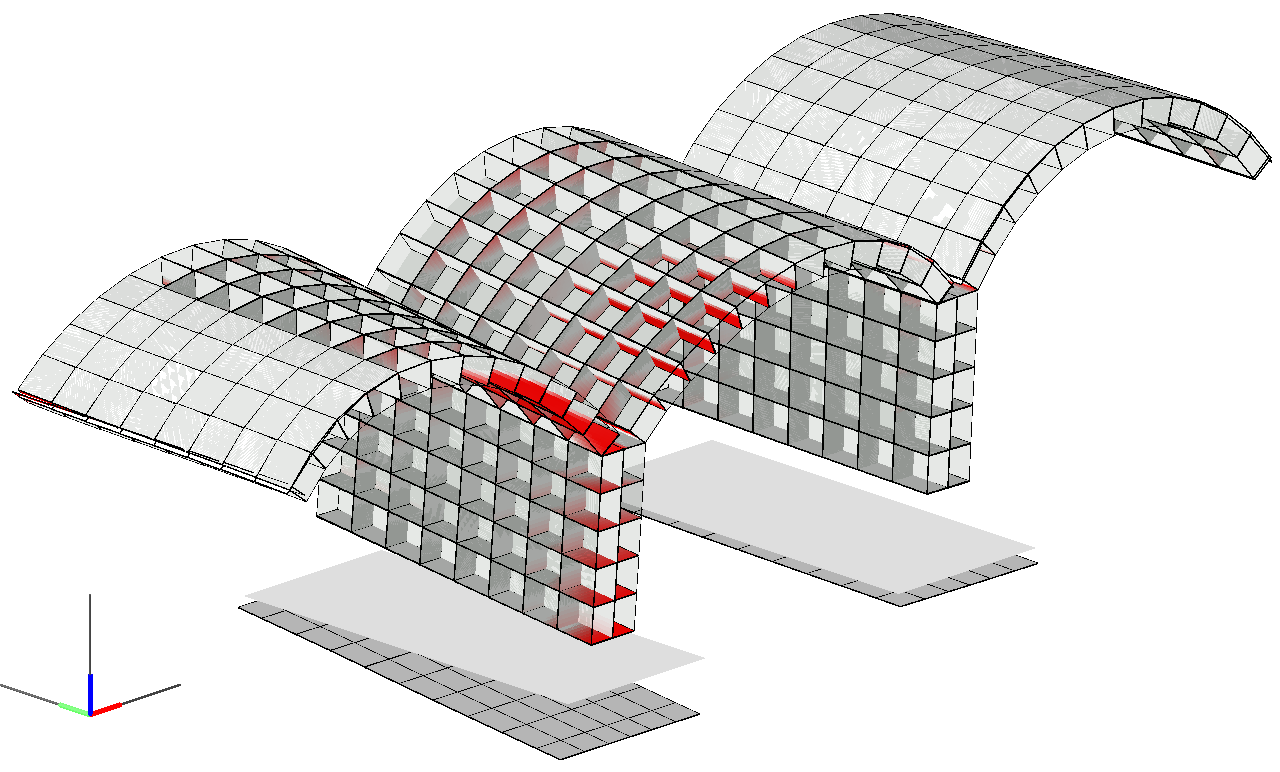
\includegraphics[width=0.42\textwidth]{./Figures/out_of_plane_scour_phases/stresses/interface_tensile_stress_3D.png} &
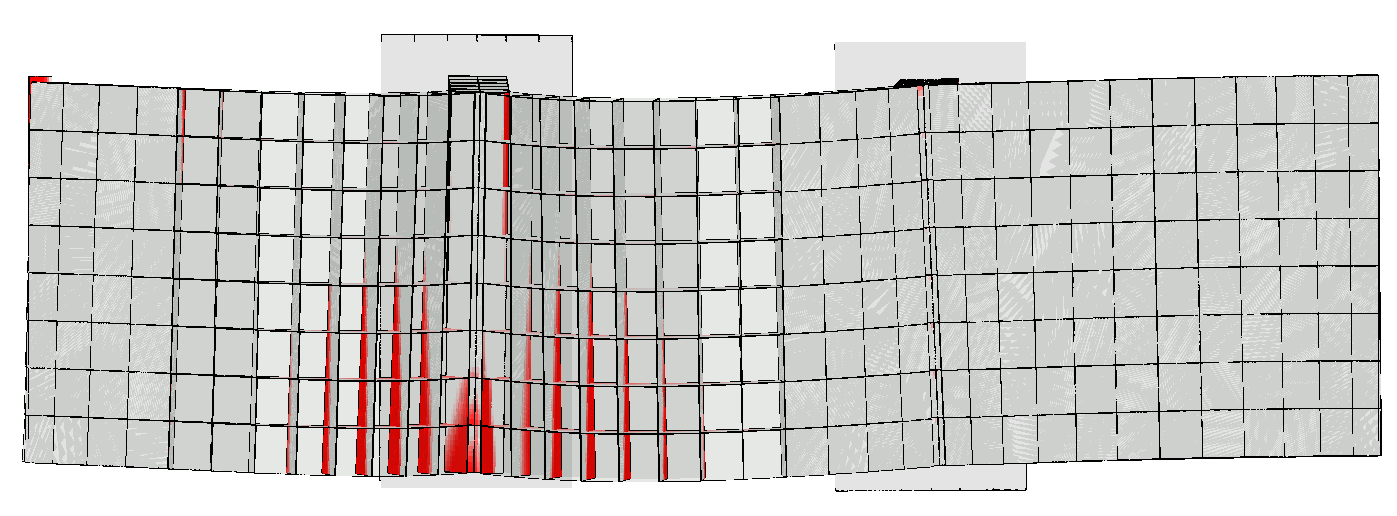
\includegraphics[width=0.42\textwidth]{./Figures/out_of_plane_scour_phases/stresses/interface_tensile_stress_XY_topview.png} \\

\textbf{Compressive stress} &
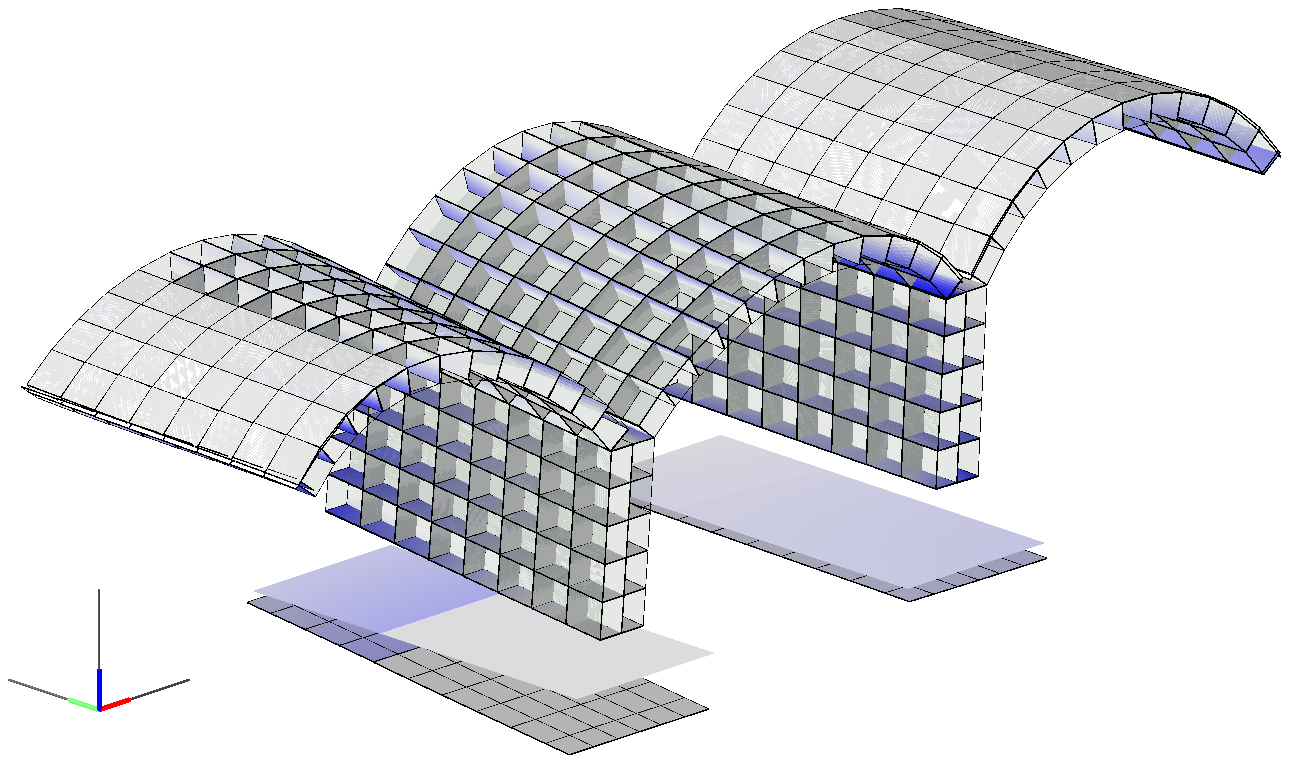
\includegraphics[width=0.42\textwidth]{./Figures/out_of_plane_scour_phases/stresses/interface_compressive_stress_3D.png} &
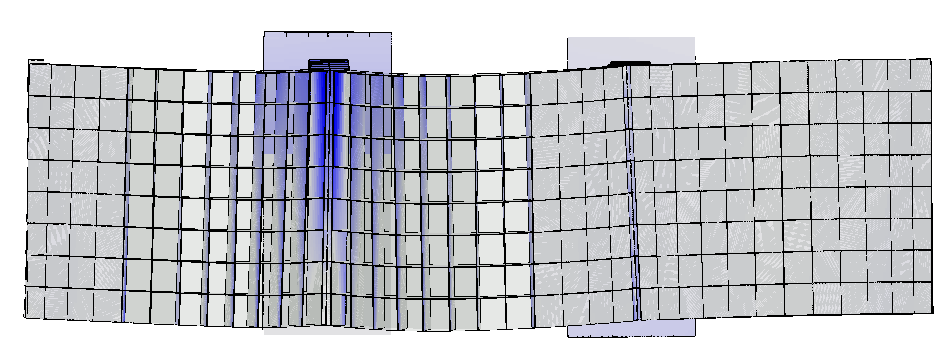
\includegraphics[width=0.42\textwidth]{./Figures/out_of_plane_scour_phases/stresses/interface_compressive_stress_XY_topview.png} \\

\end{tabular}

\caption{Interface stress distributions for the preliminary out-of-plane scour scenario, shown in 3D and XY top-view representations.}
\label{fig:dmem-scour-out-of-plane-interface-stress}
\end{figure}

\subsection{Displacement Indicator}
\label{sec:dmem-scour-out-of-plane-displacement}

\begin{figure}[htbp]
\centering
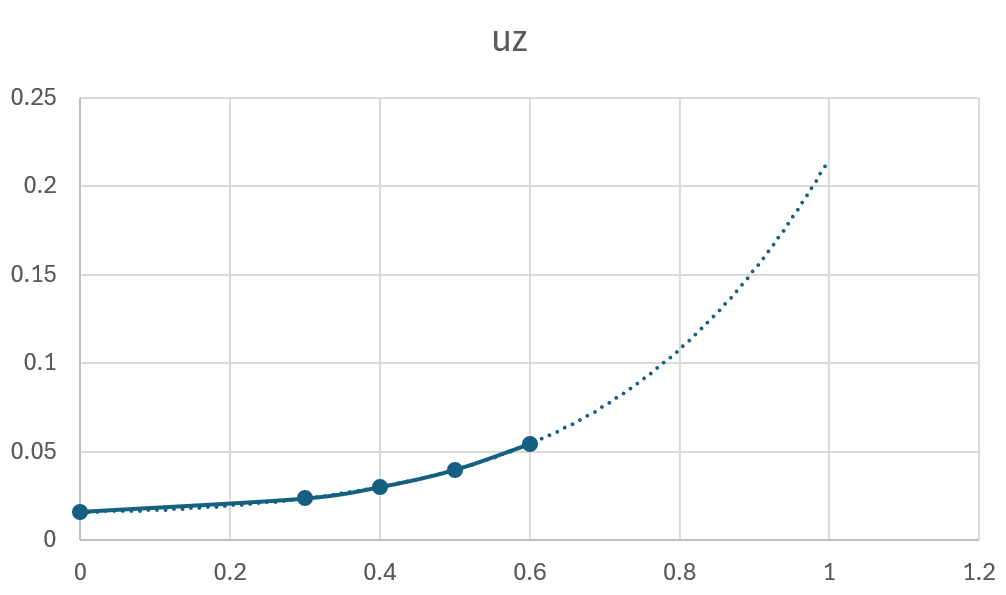
\includegraphics[width=0.82\linewidth]{./Figures/out_of_plane_scour_phases/displacement_vs_scour_ratio.png}
\caption{Displacement indicator for increasing values of the transverse scour ratio $\eta_{s,y}$.}
\label{fig:dmem-scour-out-of-plane-displacement}
\end{figure}

\Cref{fig:dmem-scour-out-of-plane-displacement} provides an initial displacement measure for the transverse scour sequence. The curve is retained as a work-in-progress result because the controlling displacement component, sign convention, and relation to residual load capacity still need to be standardised. At this stage, the figure supports the qualitative interpretation that increasing transverse support loss produces a monotonic increase in deformation demand.


% \cite{Scozzese2023}
% "
% damage mechanisms are trig-gered by levels of excavation underneath the piers of around 30% of the
% foundation base, while the system failure can be for levels even higher
% than 50% −60%, depending on the type of scour scenario (global or
% localised, respectively).
% "
% "
% Such high level of scour required to lead ma-sonry arch bridges to collapse can be explained by the significant
% robustness characterising this bridge typology.
% "